\chapter*{ERP Analysis}
\addcontentsline{toc}{chapter}{ERP Analysis}
%As proposed in \cite{schaefer_name_2011}, we computed grand average \acp{ERP} by aggregating over all trials (excluding the cue clicks) of the same stimulus from all subjects except P05 (due to the movement artifacts).
Schaefer \etal \cite{schaefer_name_2011} used very short stimuli (3.26s) allowing each stimulus to be repeated many times during during the experiment. 
This allowed them to average across hundreds of short trials. 
They then concatenated the grand average ERPs and applied a \ac{PCA}, which resulted in clearly defined spatial features. The time courses of these spatial features allowed for classification of their stimuli. We started by trying to replicate these results. 
We had fewer repetitions of our stimuli. Therefore, to preserve as much data as possible we used the full length of the trials as opposed to the first 3.26 seconds. We computed grand average \acp{ERP}s by aggregating over the full length of all trials (excluding the cue) of the same stimulus from all subjects. We then concatenated the grand average \acp{ERP} and applied a \ac{PCA}. This resulted in principle components with poorly defined spatial components \autoref{fig:components} (A and B).

In order to preserve even more of the data and we took an alternative approach and performed a \ac{PCA} on the concatenated raw trials without first calculating an average across trials. This produced clearly defined spatial components \autoref{fig:components} (C and D). Except for their (arbitrary) polarity the components are very similar across the two conditions, which replicates the results found in \cite{schaefer_name_2011}.

\begin{figure}[t] 
  \begin{center}
    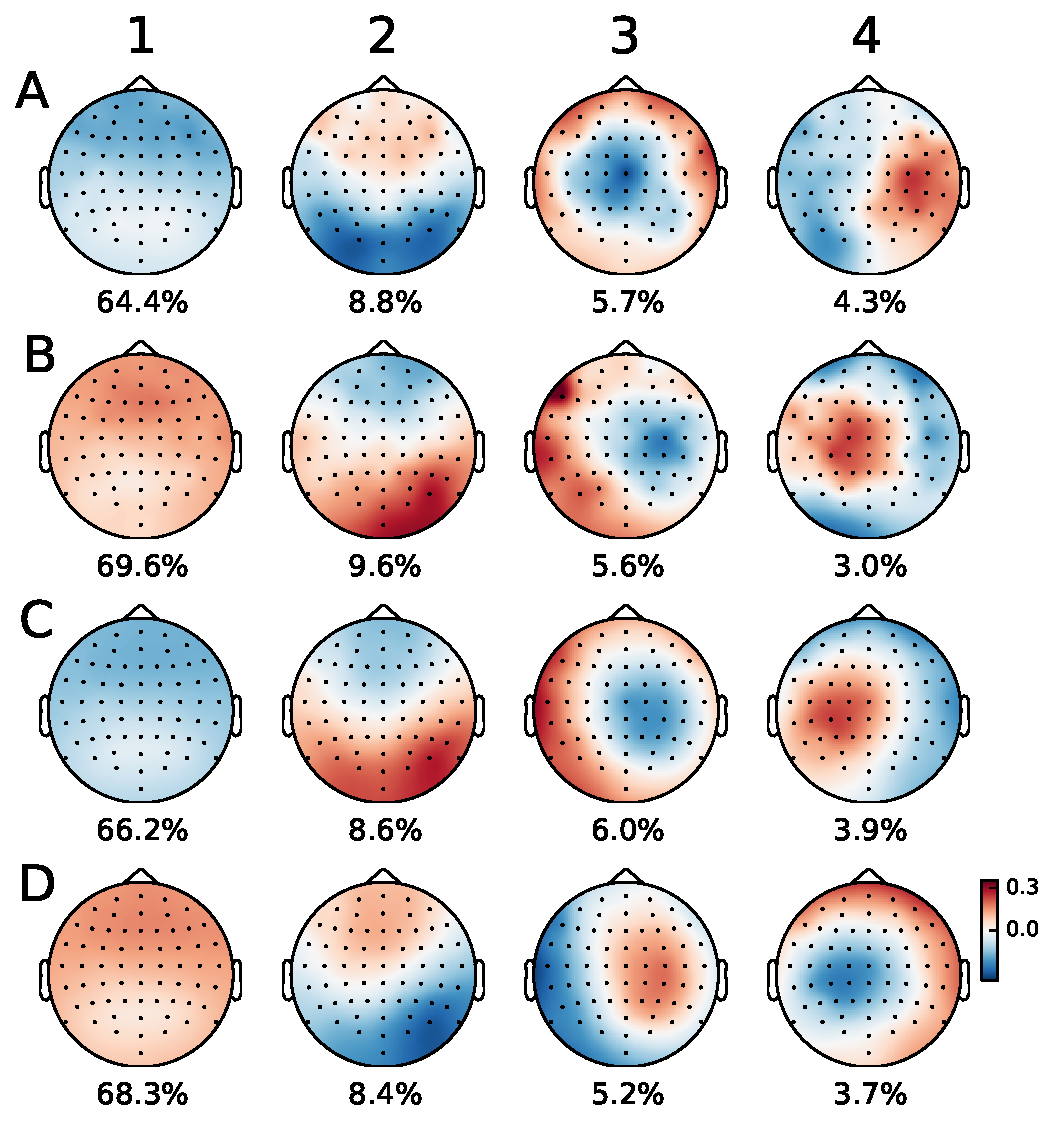
\includegraphics[width=0.8\textwidth,keepaspectratio=true]{Figures/principle_components.pdf}
%   \\\vspace{-0.8em}
    \caption{%
Topographic visualization of the top 4 principle components with percentage of the explained signal variance. %.\newline
Channel positions in the 64-channel EEG layout are shown as dots.
Colors are interpolated based on the channel weights.
%\hl{Polarity has no specific semantic.}
The PCA was computed on
\textbf{A}: the grand average \acp{ERP} of all perception trials,
\textbf{B}: the grand average \acp{ERP} of all cued imagination trials,
\textbf{C}: the concatenated perception trials,
\textbf{D}: the concatenated cued imagination trials.
}
    \label{fig:components}
  \end{center}
% \vspace{-2em}
\end{figure}

\subsection*{Component Waveform Correlations}
In order to investigate how similar the activation of these components is across conditions and stimuli we took the time course of component two over the first three seconds of each stimulus during perception and imagination and performed a correlation.
We used component two as it is accounts for the most variance and is the \hl{most topographically relevant (?)}.
The highest correlations produced by this component is r=0.32 for "Take me out to the ballagame" (\autoref{fig:ballgame}) and r=0.48 for "Eine Kleine Nachtmusic" (\autoref{fig:nachtmusic}).
Although these correlate well the perception of Eine Kleine Nachtmusic correlates well with the imagination of Jingle Bells without lyrics (r=0.30). 
The highest correlation of r=0.521 occurs between the imagination of Jingle Bells and the perception of the Star Wars theme. 

As high correlations occur in instances where they should not these results don't really tell us anything.
Table of correlations? Component 2? component 3? 

\begin{figure}[t]
  \begin{center}
    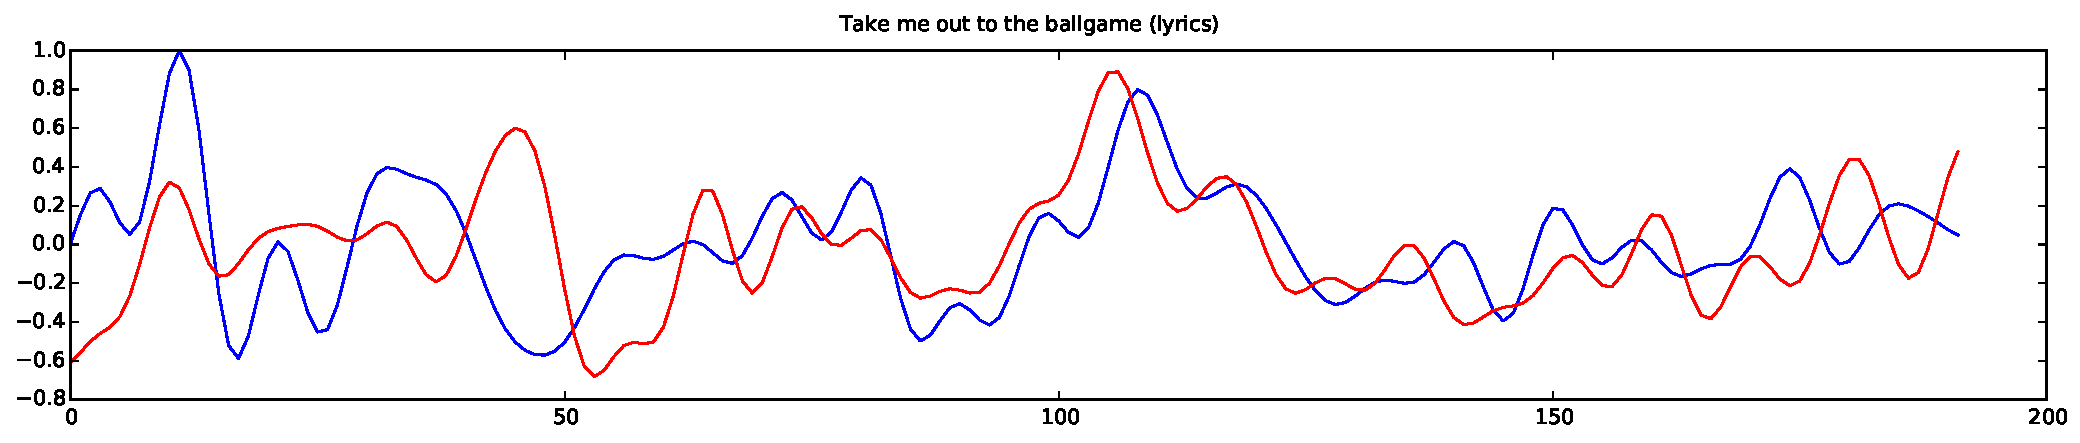
\includegraphics[width=0.8\textwidth,keepaspectratio=true]{Figures/component_timecourse_ballgame.pdf}
    \caption{
caption for this figure
}
    \label{fig:ballgame}
  \end{center}
\end{figure}

\begin{figure}[t]
  \begin{center}
    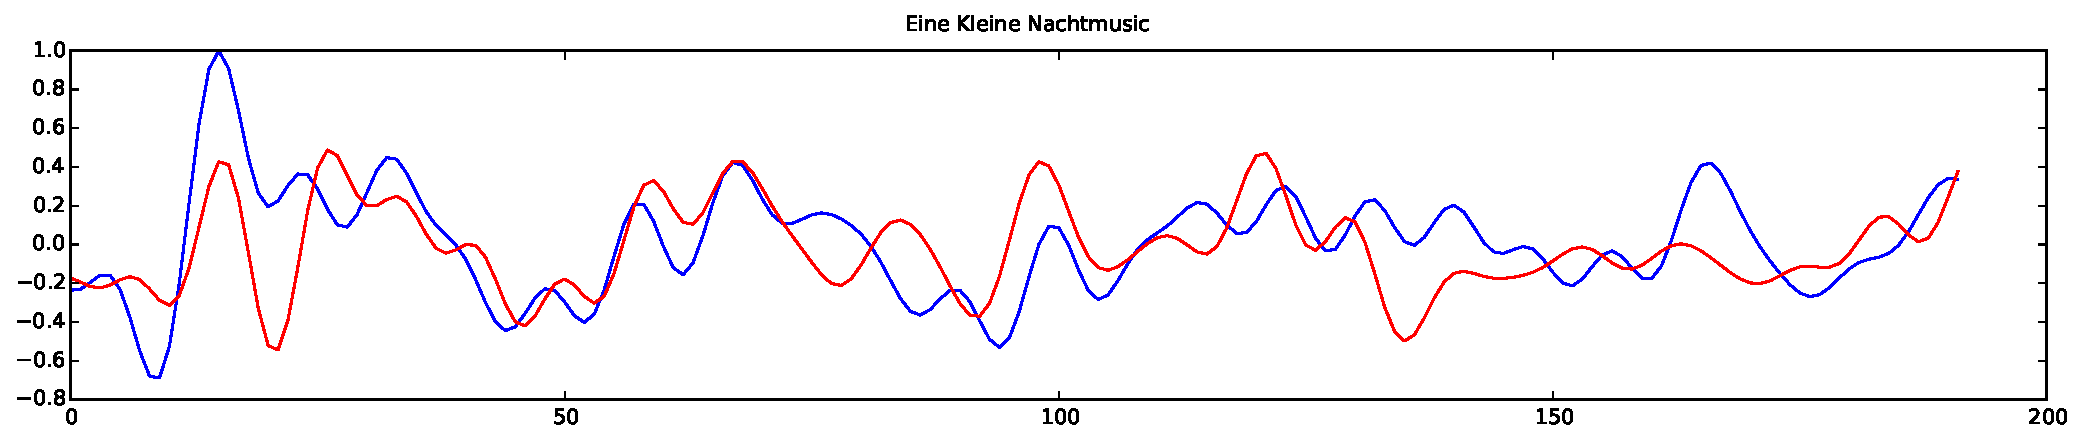
\includegraphics[width=0.8\textwidth,keepaspectratio=true]{Figures/component_timecourse_nachtmusic.pdf}
    \caption{
caption for this figure
}
    \label{fig:nachtmusic}
  \end{center}
\end{figure}